%%%%%%%%%%%%%%%%%%%%%%%%%%%%%%%%%%%%%%%%% 
% Xyz.
%
% - JLaw. 
%%%%%%%%%%%%%%%%%%%%%%%%%%%%%%%%%%%%%%%%%

%----------------------------------------------------------------------------------------
%	PACKAGES
%----------------------------------------------------------------------------------------

\documentclass[11pt]{scrartcl} % Font size.

%%%%%%%%%%%%%%%%%%%%%%%%%%%%%%%%%%%%%%%%%
% Xyz.
%
% - JLaw.
%%%%%%%%%%%%%%%%%%%%%%%%%%%%%%%%%%%%%%%%%

%----------------------------------------------------------------------------------------
%	PACKAGES
%----------------------------------------------------------------------------------------

\usepackage{listings} % Code listings with syntax highlighting.

\usepackage[english]{babel} % English hyphenation.

\usepackage{graphicx} % Insert image.
\graphicspath{{Figures/}{./}} % Specify images location.

\numberwithin{equation}{section} % Number equations within sections.
\numberwithin{figure}{section} % Number figures within sections.

\setlength\parindent{0pt} % Remove indentation from paragraphs.

\usepackage{enumitem} % List customization.
\setlist{noitemsep} % No spacing between list item.

%----------------------------------------------------------------------------------------
%	DOCUMENT MARGINS
%----------------------------------------------------------------------------------------

\usepackage{geometry} % Adjust page dimensions and margins.

\geometry{
	paper=a4paper, % Paper size.
	top=2.5cm, % Top margin.
	bottom=3cm, % Bottom margin.
	left=3cm, % Left margin.
	right=3cm, % Right margin.
	headheight=0.75cm, % Header height.
	footskip=1.5cm, % Space from bottom margin to baseline of footer.
	headsep=0.75cm, % Space from top margin to baseline of header.
}

%----------------------------------------------------------------------------------------
%	FONTS
%----------------------------------------------------------------------------------------

\usepackage[utf8]{inputenc} % Input international characters.
\usepackage[T1]{fontenc} % 8-bit encoding.

\usepackage{fourier}

%----------------------------------------------------------------------------------------
%	SECTION TITLES
%----------------------------------------------------------------------------------------

\usepackage{sectsty} % Customize section commands.

\sectionfont{\vspace{6pt}\centering\normalfont\scshape} % \section{} styling.
\subsectionfont{\normalfont\bfseries} % \subsection{} styling.
\subsubsectionfont{\normalfont\itshape} % \subsubsection{} styling.
\paragraphfont{\normalfont\scshape} % \paragraph{} styling.

%----------------------------------------------------------------------------------------
%	HEADERS AND FOOTERS
%----------------------------------------------------------------------------------------

\usepackage{scrlayer-scrpage} % Customize headers and footers.

\ohead*{} % Right header.
\ihead*{} % Left header.
\chead*{} % Centre header.

\ofoot*{} % Right footer.
\ifoot*{} % Left footer.
\cfoot*{\pagemark} % Centre footer. % Include structure.

%----------------------------------------------------------------------------------------
%	TITLE 
%----------------------------------------------------------------------------------------

\title{	
	\normalfont\normalsize
	\textsc{Org}\\ % Accent header.
	\vspace{25pt}
	\rule{\linewidth}{0.5pt}\\
	\vspace{20pt}
	{\huge Template}\\ % Main title.
	\vspace{12pt}
	\rule{\linewidth}{2pt}\\
	\vspace{12pt} 
}

\author{\LARGE JLaw}

\date{\normalsize\date}

\begin{document}

\maketitle % Print title.

%----------------------------------------------------------------------------------------
%	FIGURE
%----------------------------------------------------------------------------------------

\section{Image}

\begin{figure}[h]
	\centering
	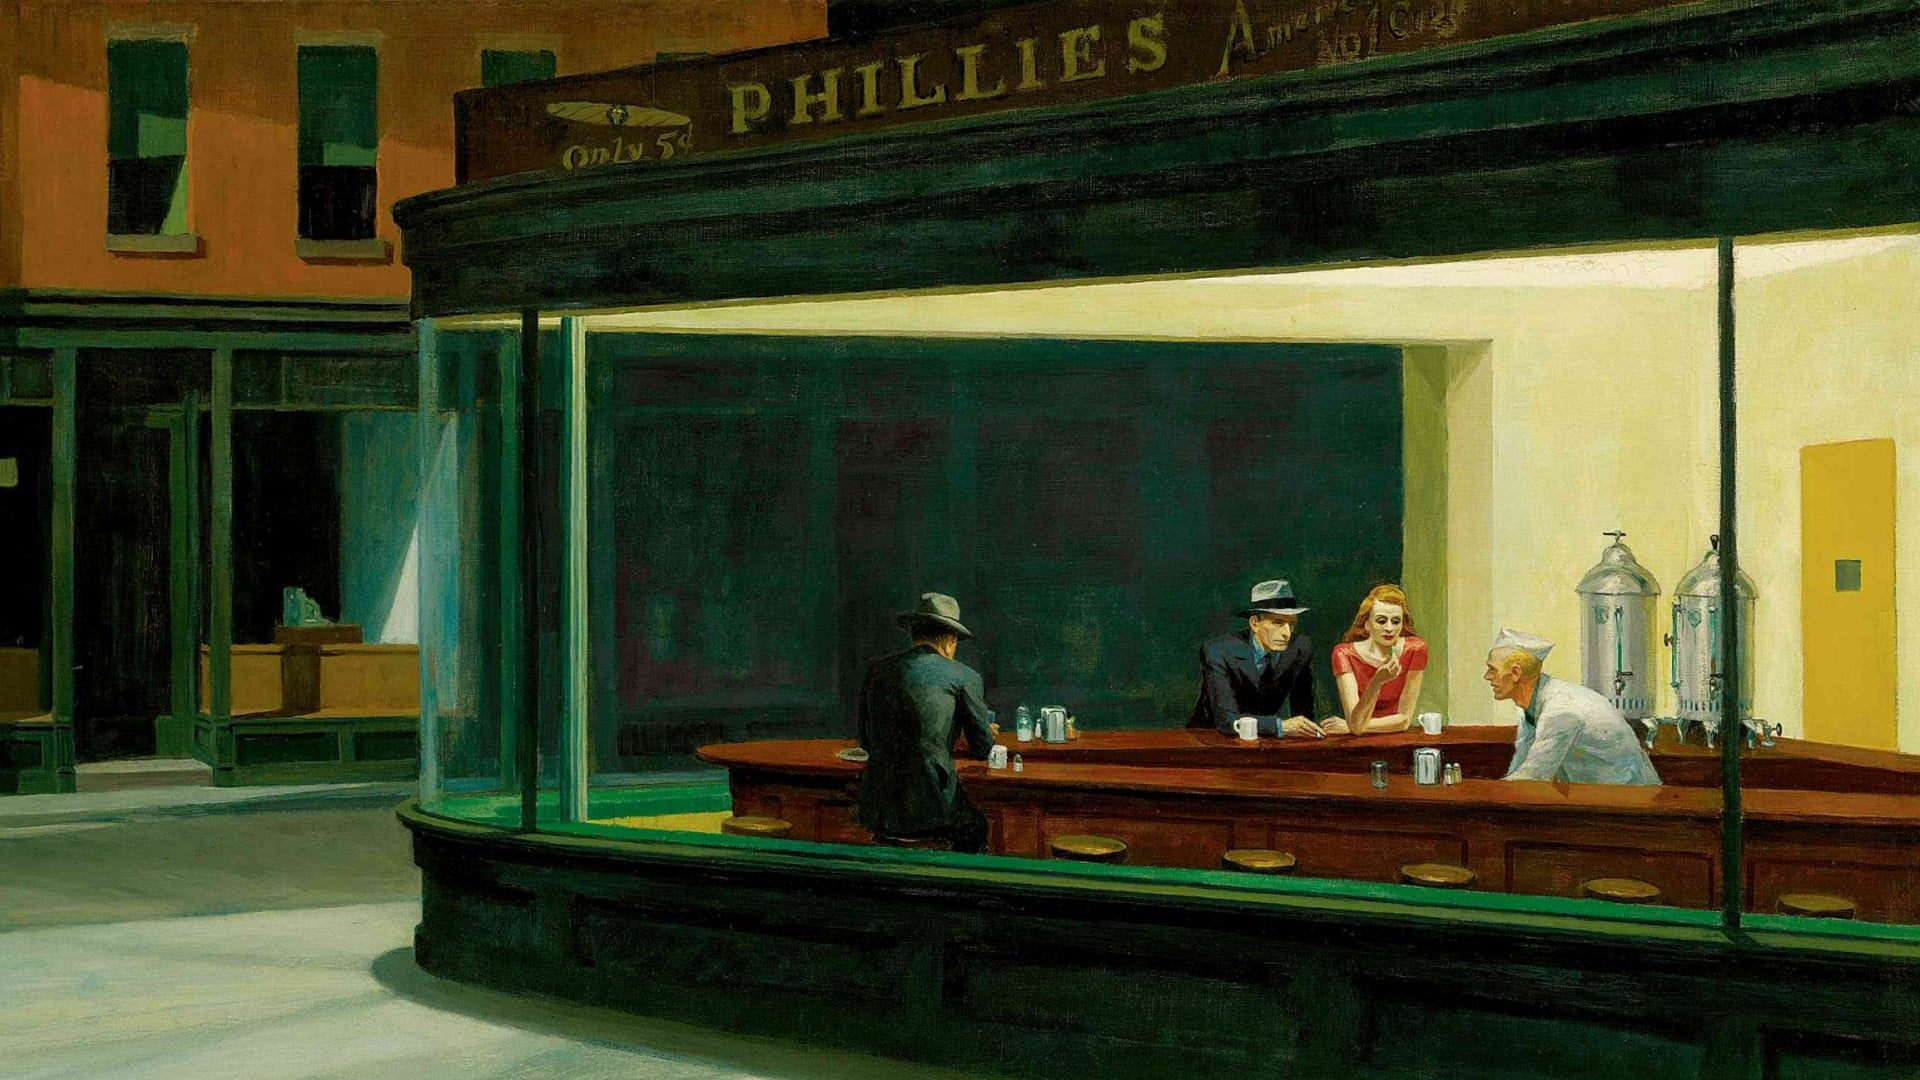
\includegraphics[width=0.5\columnwidth]{nighthawk.jpg}
	\caption{desc.}
\end{figure}

%----------------------------------------------------------------------------------------
%	SECTION 1
%----------------------------------------------------------------------------------------

\section{Header}

\subsection{Sub-sec}

%------------------------------------------------

\subsubsection{Sub-sub-sec}

xyz.

%------------------------------------------------

\subsubsection{Sub-seb-sec2}

xyz.

%------------------------------------------------

\paragraph{Para}

xyz.

%----------------------------------------------------------------------------------------
%	SECTION 2
%----------------------------------------------------------------------------------------

\section{Header}

\lstinputlisting[
	caption=xyz., % Caption.
	label=lst:zyx, % Reference label.
	language=Solidity, % Use Sol functions/syntax highlighting.
	frame=single,
	showstringspaces=false, 
	numbers=left, % Line numbers.
	numberstyle=\tiny, % Line number styling.
	]{xyz.sol}

%------------------------------------------------

\subsection{Sub-sec}

Xyz.

%------------------------------------------------

\end{document}